\subsection{第 6 课}

\subsubsection{脑图}

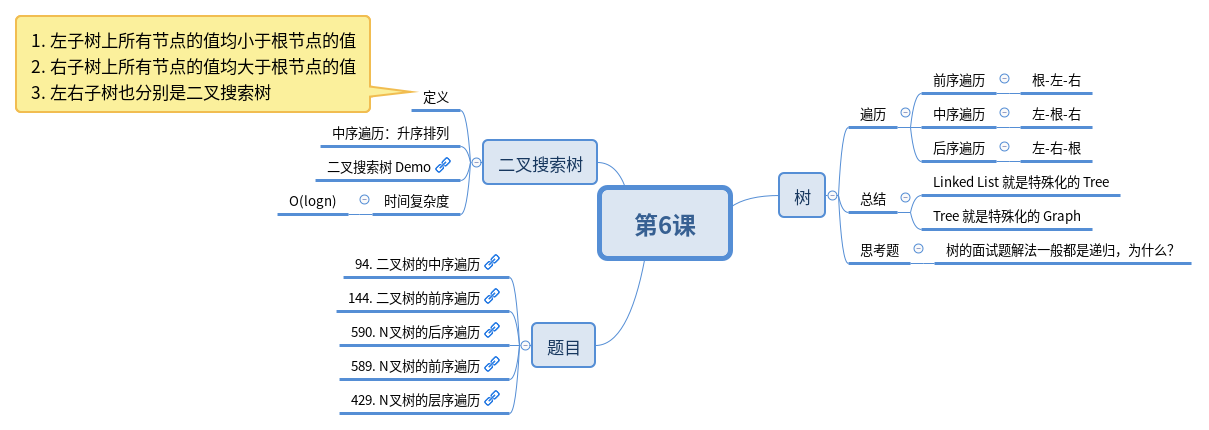
\includegraphics[width=170mm,height=80mm]{images/第6课.png}

\subsubsection{题目}

\begin{itemize}
  \item \hyperref[leetcode:94]{94. 二叉树的中序遍历}
  \item \hyperref[leetcode:144]{144. 二叉树的前序遍历}
  \item \hyperref[leetcode:590]{590. N叉树的后序遍历}
  \item \hyperref[leetcode:589]{589. N叉树的前序遍历}
  \item \hyperref[leetcode:429]{429. N叉树的层序遍历}
\end{itemize}
